Several files (dynamic libraries, executables, drivers) were analyzed and reversed in order to achieve the aforementioned goals. However, the main analysis was performed in the {\bfseries ntoskrnl.exe} file, which is the one holding the actual implementation of the Windows Kernel.

It's important to stress that most of the general analysis was carried out using the Basic level of Telemetry. 

Further sections will depict different challenges and achievements faced during the analysis.

\section{Understanding how Telemetry makes use of ETW}
Where, who and what were some of the questions that needed to be answered in order to be able to get information about the providers that were registered against the DiagTrack session. 
It's possible to obtain the whole list of providers registered to a particular session, by executing the following powershell command: 

\begin{figure}[H]
  \begin{lstlisting}
    Get-EtwTraceProvider | where {$_.SessionName -match "<SESSION_NAME>"}
  \end{lstlisting} 
  \caption[]{Powershell comand to list ETW providers registered against a particular session. }
  \label{fig:powershell_cmd}
\end{figure}

One way to answer all the aforementioned questions, was to intercept the moment when some provider was going to write a message. If a breakpoint was set at that exact moment, it would be possible to gather information such as: 
\begin{enumerate}
\item The piece of code that triggered the write (by inspecting the call stack of the function).
\item The actual content of the log being written.
\end{enumerate} 
However, the function being used for executing writes ({\bfseries EtwWrite}) was not just used by the providers attached to the DiagTrack session but also by all the providers using the ETW framework. It was necessary to find a way to filter them and only intercept the ones important for the analysis. 

Using \ref{powershell_cmd}, it was possible to extract a GUID's list of the providers that were attached to the DiagTrack session. With this information, it would be possible to make the breakpoint to be triggered only when the provider's GUID that was trying to write was in the list. 

Nevertheless, this strategy had one minor issue. The function ({\bfseries EtwWrite}) had five parameters and none of them would show directly the GUID:

\begin{figure}[H]
  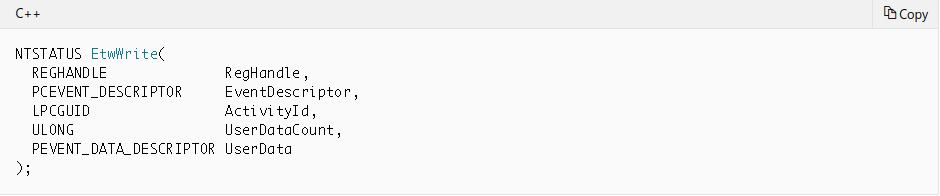
\includegraphics[width=\linewidth]{images/etw_write_docu.png}
  \caption[]{Documentation for EtwWrite function \footnote{https://docs.microsoft.com/en-us/windows-hardware/drivers/ddi/content/wdm/nf-wdm-etwwrite}. }
  \label{fig:etw_write_docu}
\end{figure}

The first parameter is the registration handler. This object is returned once the provider executed the registration ({\bfseries EtwRegister)} successfully.
On the other hand, the {\bfseries EtwRegister} receives the GUID as parameter:
\begin{figure}[H]
  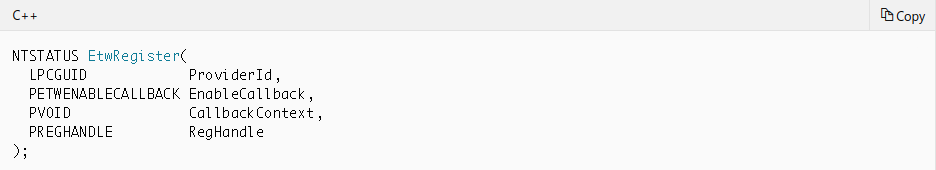
\includegraphics[width=\linewidth]{images/etw_register_docu.png}
  \caption[]{Documentation for EtwRegister function \footnote{https://docs.microsoft.com/en-us/windows-hardware/drivers/ddi/content/wdm/nf-wdm-etwregister}.}
  \label{fig:etw_register_docu}
\end{figure}

Therefore, in order to perform the cross-check it was not enough with information from the {\bfseries EtwWrite} function, but also information from the {\bfseries EtwRegister} was needed. To summarize, to understand if the write was being done by a provider registered against the DiagTrack session it was necessary to: 
\begin{enumerate}
    \item Extract the whole list of providers registered attached to the DiagTrack session.
    \item Intercept all the {\bfseries EtwRegister} executions and check if the GUID being used was inside the list.
    \item If it was, save the handler. 
    \item Intercept all the {\bfseries EtwWrite} executions and check if the handler being used is one of the stored handlers.
    \item If it was, the provider that is writing, is attached to the DiagTrack session.
\end{enumerate}

Even though the strategy seemed to be theoretically promising, it was necessary to understand how to actually carry out these actions. Further sections will depict that process.

\subsection{Reversing registration process}

The first step was, using {\bfseries IDA} \ref{IDA}, analyze the {\bfseries EtwRegister} function. The dissasembly of the function  that the only action being performed was calling a second function named {\bfseries EtwpRegisterProvider}. 

\begin{centering}
\begin{figure}[H]
  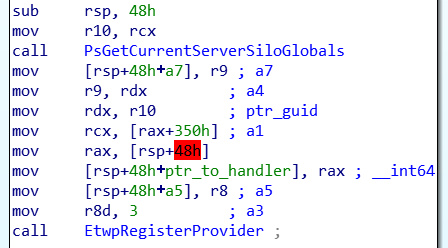
\includegraphics[width=12cm]{images/etwRegister_code.png}
  \caption[]{Dissasembly of ETWRegister function}
  \label{fig:etwRegister_code}
\end{figure}
\end{centering}

A quick and vague analysis of it, showed that, apparently, {\bfseries EtwpRegisterProvider} holded the actual implementation of the registration process. However, due to the lack of documentation regarding this function, it was necessary to understand in a mode in-depth way what was actually happening. In order to explain what actions were performed in a better way, lets split it two parts:
\begin{itemize}
  \item Check if a GUID for this provider already exists.
  \item If not, create a new one. 
\end{itemize}

\subsubsection{Check if GUID for this provider already exists}
At this point, the layout of the GUID structure was totally unknown. 

After performing some sanity checks, the {\bfseries EtwpRegisterProvider} tries to get a pointer to the GUID structure. This whole part is basically implemented inside another function called {\bfseries EtwpFindGuidEntryByGuid}. It receives 3 parameters:


\newpage
{\huge 1. We couldn't ensure that the data was being written was actually going to the DiagTrack session .}

\section{When and how providers are registered}
\section{How writes are carried out}
\section{Relation between ETW session and ETW providers}
\section{Identifying the buffers}
\section{Provider GUID vs Group Provider GUID}
\section{Checking correctness of logged events}
\section{Automatization of event logging}
\section{Service isolation}
\section{Triggers}
\section{searching for new triggers} YARA
\section{Difference among configuration levels of telemtry}
\section{Analysis of sent data over the channel to Microsfot backend services}
